\chapter{Rectangular Waveguide (1)}
Our previous chapter dealt with the propagation of an electromagnetic wave through a rectangular and cylindrical waveguide. it took a general approach in analyzing waveguides, where derivations for equations for the propagation of the electromagnetic wave in cylindrical waveguides were considered in lossless conditions. Illustrations for two special cases, the transverse electric mode (TE) and the transverse magnetic modes (TM) were made. We had the following formulas in equations~\ref{eqn:transverseex}-\ref{eqn:transversehy} derived for the TE and TM modes, rewritten as:
\begin{align*}
E_x = -\frac{j\omega\mu}{h^2}.\frac{\partial H_z}{\partial y} - \frac{j\beta}{h^2}.\frac{\partial E_z}{\partial x}\\
E_y = \frac{j\omega\mu}{h^2}.\frac{\partial H_z}{\partial x} - \frac{j\beta}{h^2}.\frac{\partial E_z}{\partial y}\\
H_x = \frac{j\omega\epsilon}{h^2}.\frac{\partial E_z}{\partial y} - \frac{j\beta}{h^2}.\frac{\partial H_z}{\partial x}\\
H_y = -\frac{j\omega\epsilon}{h^2}.\frac{\partial E_z}{\partial x} - \frac{j\beta}{h^2}.\frac{\partial H_z}{\partial y}
\end{align*}

In this chapter we are concerned with the propagation and derivation of these parallel waves in a rectangular waveguide referred to as TE and TM modes, using the same general approach in waveguide analysis.
\begin{figure}[h]
\centering
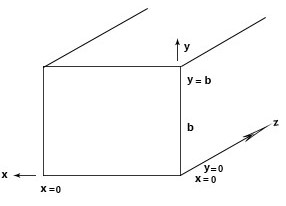
\includegraphics[width=0.7\linewidth]{./graphics/lec38fig1}
\caption{A Rectangular Waveguide}
\label{fig:lec38fig1}
\end{figure}
The waveguide in figure~\ref{fig:lec38fig1} shows the x, y and z coordinates in which the electromagnetic wave is propagated. It is propagated along the z direction. $a$ is the width of the guide while the $b$ is the breadth of the guide. In this guide $a \leq b$.

Considering the transverse magnetic (TM mode), $ E_{z} = 0$, $H_{z} = 0 $ longitudinal components. For a transverse field to exist, either $ E_{z} $ or $ H_{z} $ has to be zero. $ H_{z} $ is oriented on the transverse plane and $ E_{z} $ on the longitudinal plane.

Now we first find the solution of the longitudinal component $ E_{z} $ and then find the transverse component $ H_{z} $, and then we apply an initial condition to it. Let us consider the wave equation.
\begin{equation}
\nabla^{2}\bar{E_{z}} + \omega^{2}\mu\epsilon_{o}\bar{E_{z}} = 0
\end{equation}
$ \omega $  is the frequency of the wave, $ \mu $   is the permeability of the medium, $ \epsilon $ is the permittivity of the medium filling the waveguide. We expand $ \nabla^{2} $ in the cartesian coordinate system.
\begin{equation}
\frac{\partial ^{2} E_z}{\partial x^2} + \frac{\partial ^2 E_z}{\partial y^2} + \frac{\partial ^2 E_z}{\partial z^2}+ \omega^2\mu\epsilon {E_{z}} = 0
\label{eqn:maxwellele}
\end{equation}
We now solve by the separation of variables.
%\begin{figure}
%\centering
%\includegraphics[width=0.7\linewidth]{./graphics/onej}
%\caption{wave propagation along z}
%\label{fig:one}
%\end{figure}
\begin{equation}
E_z (x,y,z) = X(x)Y(y)Z(z)
\label{eqn:electricwave}
\end{equation}
Substitute equation~\ref{eqn:electricwave} into equation~\ref{eqn:maxwellele}
\begin{align}
YZ \frac{\partial ^{2} X}{\partial x^2} + XZ \frac{\partial ^2 Y}{\partial y^2} + XY \frac{\partial ^2 Z}{\partial z^2}+ \omega^2\mu\epsilon {XYZ} = 0
\end{align}
Divide through by XYZ.
\begin{align}
\frac{1}{X}\frac{\partial ^{2} E_z}{\partial x^2} + \frac{1}{Y}\frac{\partial ^2 E_z}{\partial y^2} + \frac{1}{Z} \frac{\partial ^2 E_z}{\partial z^2} + \omega^2\mu\epsilon {E_{z}} = 0
\end{align}
This tells us that the wave is propagated in both the x, y and z directions inside the waveguide. 

Let,  
\begin{align*}
\frac{1}{X}\frac{\partial^2 X}{\partial x^2} = -A^2\\
\frac{1}{Y}\frac{\partial^2 Y}{\partial y^2} = -B^2\\
\frac{1}{Z}\frac{\partial^2 Z}{\partial z^2} = -\beta^2
\end{align*}

Being a second-order homogeneous equation,   
\begin{align*}
X(x) = C_{1}cos A_{x} + C_{2}sin A_{x}\\
Y(x) = C_{3}cos B_{x} + C_{4}sin B_{x}\\
Z(x) = C_{5} e^{-j \beta z} + C_{6} e^{+j \beta z}
\end{align*}                                  
The cosine and sine functions show amplitude variation which is a standing wave kind of behaviour. The $C_{5}e^{+j\beta z}$ and $C_{6}e^{-j\beta(z)}$ are travelling waves in the positive and negative z direction respectively. 
Which indicates their forward and backward travelling waves.
Therefore, by substituting the above equations into equation~\ref{eqn:electricwave} we can then write the general equation for the component $E_{z}$.
\begin{equation*}
E_{z} = C_{5}(C_{1}cos A_{x} + C_{2}sin A_{x})(C_{3}\cos B_{y} + C_{4}sin B_{y}) e^{-j\beta z}
\end{equation*}
Now we apply the boundary condition on $E_{z}$ to obtain the constants. $E_{z}$ = 0 at  

\begin{enumerate}[(i)]
\item x = 0, x = a
\item y = 0, y = b
\item x = 0, $ C_{1} $ = 0
\item y = 0, $ C_{3} $ = 0
\end{enumerate}     
\begin{align*}
E_{z} = C_{5}C_{2}C_{4}\sin A_{x}\sin B_{y} e^{-j\beta z}
\end{align*}
Let C = $ C_{5}C_{2}C_{4} $
\begin{equation}
E_{z} = C\sin A_{x}\sin B_y e^{-j\beta z}
\label{eqn:elesoln}
\end{equation}
For $x = a$ and $y = b$ we get,
\begin{align*}
A_xa = m\pi\\
A_x = \frac{m\pi}{a}\\
B_yb = n\pi\\
B_y = \frac{n\pi}{b}
\end{align*}
Substitute $A_x$ and $B_y$ into equation~\ref{eqn:elesoln}.
\begin{align*}
E_{z} = C sin\frac{m\pi}{a} sin\frac{n\pi}{b} e^{-j\beta z}
\end{align*}
$m$ index is field variation in broader (a) dimension, and $n$ index is field variation in shorter (b) dimension. If $m$ is taken as 1, we have one circle variation. If two, we have two circles variation. $T_{mn}$ values tell us the number of half circles in the magnetic field. When $m = n = 0$, then the field goes to zero, as such the field does not exist. Substitute equatio~\ref{eqn:elesoln} into equation~\ref{eqn:electricwave}.
\begin{align*}
-\frac{m\pi}{a} - \frac{n\pi}{b} - \beta^{2} + {\omega^2\mu\epsilon} = 0
\end{align*}
\begin{equation}
\beta = \sqrt{{\omega^2\mu\epsilon} - \frac{m\pi}{a} - \frac{n\pi}{a}}
\label{eqn:dispersionrelatn}
\end{equation}
This equation is called the dispersion relation\index{Dispersion Relation}. It tells us how the velocity of the phase constant varies as a function of the frequency of the structure. by this, we can say that if either $m$ or $n$ is made zero. We can find $h$ by substituting the dispersion relation in equation~\ref{eqn:h}.
\begin{dmath*}
h^{2} = \omega^2\mu\epsilon - \beta^{2} = -\frac{m\pi}{a} - \frac{n\pi}{b}
\end{dmath*} 

\section{Tranverse Magnetic ($TM$) Mode}\index{Transverse Magnetic Mode}
Considering the various modes of transmission of electromagnetic waves, the $TM_{00}$ mode does not exist and also the $TM_{mo}$ does not exist still. $TM_{11}$ is the lowest order of TM mode which can exist on the waveguide. The $TM_{00}$ and $TM_{m0}$ are zero because if they are substituted into the general wave equation the transverse field cannot exist. 

Now we substitute, $H_{z} = 0$, into equations~\ref{eqn:transverseex}-\ref{eqn:transversehy} and then we substitute $\dfrac{\partial E_{z}}{\partial{x}}$ for $\dfrac{m \pi}{a}$ in the case of $TM_{11}$. 
\begin{dmath*}
E_x = -\frac{j \beta}{h^2}.\frac{\partial E_{z}}{\partial{x}} = -\frac{j \beta}{h^{2}}\cdot\left(\frac{m\pi}{a}\right) C\cos \left(\frac{m\pi x}{a}\right)\sin \left(\frac{n\pi y}{b}\right)e^{-j \beta z}
\end{dmath*}
\begin{dmath*}
E_y = -\frac{j \beta}{h^2}\frac{\partial E_{x}}{\partial{y}} = -\frac{j \beta}{h^{2}}\left(\frac{n\pi}{b}\right) C \sin\left(\frac{m\pi x}{a}\right)\cos \left(\frac{n\pi y}{b}\right)e^{-j \beta z}
\end{dmath*}
\begin{dmath*}
H_x = \frac{j \omega\epsilon}{h^2}\cdot\frac{\partial E_{z}}{\partial{y}} = \frac{j \omega\epsilon}{h^{2}}\cdot\left(\frac{n\pi}{a}\right) C \sin \left(\frac{m\pi x}{a}\right)\cos \left(\frac{n\pi y}{b}\right)e^{-j \beta z}
\end{dmath*}
\begin{dmath*}
H_y =-\frac{j \omega\epsilon}{h^2}\frac{\partial E_{z}}{\partial{x}} = -\frac{j \omega\epsilon}{h^{2}}\left(\frac{m\pi}{b}\right) C \cos \left(\frac{m\pi x}{a}\right)\sin \left(\frac{n\pi y}{b}\right)e^{-j \beta z}
\end{dmath*}		      
%\begin{figure}
%\centering
%\includegraphics[width=0.7\linewidth]{./graphics/fivej}
%\caption{TM mode patterns}
%\label{fig:five}
%\end{figure}

If we these on a waveguide plot, we will have both the electric field, $E_{y}$, and the magnetic wave field, $H_{x}$, which is x-oriented. $H_{y}$ component is maximum on the y-axis when tangential to the boundary. Similarly, when the magnetic field $H_{x}$ is maximum on the x-axis when the magnetic field is maximum and tangential to the conducting boundary, that is where the electric field is zero when it is tangential to the conducting boundary.

\section{Transverse Electric mode ($TE$) mode}\index{Transverse Electric Mode}
For $E_{z} = 0$ and $H_{z}$, we substitute $E_{z} = 0$ into equations~\ref{eqn:transverseex}-\ref{eqn:transversehy}, still and solve and solve the routine same algebra as usual to obtain the magnetic field.
\begin{equation}
H_z = C\cos\left(\frac{m\pi x}{a}\right) \cos\left(\frac{n\pi y}{b}\right)e^{-j\beta z}
\end{equation}
This is the equation we are looking for because we can verify when x is equal to zero ($x = 0$), the fields are maximum also when the y is equal to zero and to the value of b respectively, i.e. $y = 0$ and $y = b$, again the fields are maximum. This is what we are looking for, that the tangential component of electromagnetic field must be maximum.